\section{Motivating Example}
\label{sec:motivating-example}

In this section, we illustrate how \textsc{MockDetector} finds mock invocations in unit tests. Our tool identifies invocations on variables which have been assigned an object flowing from a mock creation site either using a forward dataflow may-analysis (Soot-based analysis) or by solving specified declarative constraints (Doop-based analysis).

% explain focal methods first.

To motivate our work, consider Listing~\ref{lis:mockCall}, which presents a unit test case from the Maven project. Line~\ref{line:mock} calls \textit{getRequest()}, invoking it on the mock object \texttt{session}. Line~\ref{line:real} then calls \textit{getToolchainsForType()}, which happens to be the focal method whose behaviour is being tested in this test case. At the bytecode level, the two method invocations are indistinguishable with respect to mockness; to our knowledge, current static analysis tools cannot easily tell the difference between the method invocation on a mock object on line~\ref{line:mock} and the method invocation on a real object on line~\ref{line:real}. Given mockness information, an IDE could provide better suggestions. And the uncertainty about mockness would confound a naive static analysis that attempts to identify focal methods. For instance, Ghafari et al~\cite{ghafari15:_autom}'s heuristic would fail on this test, as it returns the last mutator method in the object under test, and the focal method here is an accessor. 

\paragraph{Basic dataflow analysis} The dataflow analysis based \textsc{MockDetector} implementation maintains an abstraction mapping values (local variables or field references) in the Jimple intermediate representation (IR) to \texttt{MockStatus}, which holds three bits monitoring each value's status being a mock, a mock-containing array, and a mock-containing collection, respectively. The declarative version, which we do not explain in this section, maintains relations that track the same bits.

Figure~\ref{fig:focalMethodIllustration} shows how our dataflow analysis works. We begin with an empty abstraction (no mapping for any values, equivalent to all bits false for each value) before line 2. For the object creation on line 2, since the call to the no-arg \texttt{Object} constructor is not one of our hardcoded mock APIs, our analysis does not declare \texttt{object1} to be a mock object. In practice, our abstraction simply does not create an explicit binding for \texttt{object1}, instead leaving the mapping empty as it was prior to line 2; but it would be equivalent to create a new \texttt{MockStatus} with all bits false and bind it to \texttt{object1}. Thus, continuing to line 5, we see that the invocation \texttt{object1.foo()} is not known to be a mock invocation. Tying back to our focal methods application, we would not exclude the call to \texttt{foo()} from being a possible focal method.

On the other hand, our imperative analysis sees the mock creation API \texttt{java.lang.Object mock(java.lang.Class)} on line 8. It thus adds a mapping from local variable \texttt{object2} to a new \texttt{MockStatus} with the mock bit set to true. When the analysis reaches line 11, because \texttt{object2} has a mapping in the abstraction with the mock bit being set, \textsc{MockDetector} will deduce that the call on line 11 is a mock invocation. This implies that the call to method \textit{foo()} on line 11 cannot be a focal method.

\paragraph{Extensions: arrays and collections} While we were designing \textsc{MockDetector}, we observed several cases where developers store mock objects in arrays and collections. Listing~\ref{lis:container} presents method \textit{setUp()} in class \texttt{NodeListIteratorTest} from commons-collections-4.4, where line \ref{line:storeMocksInArray} puts the mock \texttt{Node} objects in the array-typed field \texttt{nodes}. This field is later used in test cases. To find arrays containing mock objects, our analysis would first locate assignment statements containing array references, and would gather all the local variables or field references which appear as sources in these statements. It then checks whether any of these local variables or field reference sources have been marked as mock objects in the analysis. If so, then the tool would mark the local variable or field reference representing the array as an array mock---it propagates the mockness to this array container.

Figure~\ref{fig:arrayMockIllustration} illustrates the process of identifying a mock-containing array. As \textsc{MockDetector} finds a Mock API on line 2, it stores \texttt{object1}'s Jimple IR with MockStatus setting mock bit to 1 into the abstraction. When analysis iterates to line 5, \textsc{MockDetector} finds an array reference, along with \texttt{object1} stored in the array at right hand side of the assignment statement. It finds \texttt{object1}'s Jimple IR in the abstraction's key set, with the mock bit turned on. It can now deduce that \textsc{objects} at the left hand side must represent an array container holding at least one mock object. Therefore, \textsc{MockDetector} puts \textsc{objects}' Jimple IR mapped to a MockStatus setting mock-containing array bit (named arrayMock flag) turned on into the abstraction. 

\lstset{language=java,
    keywordstyle=\color{blue}\bfseries,
    commentstyle=\color{green},
    stringstyle=\ttfamily\color{red!50!brown},
        showstringspaces=false}
\lstset{literate=%
    *{0}{{{\color{red!20!violet}0}}}1
    {1}{{{\color{red!20!violet}1}}}1
    {2}{{{\color{red!20!violet}2}}}1
    {3}{{{\color{red!20!violet}3}}}1
    {4}{{{\color{red!20!violet}4}}}1
    {5}{{{\color{red!20!violet}5}}}1
    {6}{{{\color{red!20!violet}6}}}1
    {7}{{{\color{red!20!violet}7}}}1
    {8}{{{\color{red!20!violet}8}}}1
    {9}{{{\color{red!20!violet}9}}}1
}

\begin{lstlisting}[basicstyle=\ttfamily, caption={This code snippet illustrates an example from maven-core, where both the focal method \texttt{getToolchainsForType} and a method invocation \texttt{getRequest} on a mock object occur in test \textit{testMisconfiguredToolchain()}},
basicstyle=\scriptsize\ttfamily,language = Java, framesep=4.5mm, escapechar=|,
framexleftmargin=1.0mm, captionpos=b, xleftmargin=3.5ex, label=lis:mockCall]
@Test
public void testMisconfiguredToolchain()
                 throws Exception {
    MavenSession session = mock( MavenSession.class );
    MavenExecutionRequest req = 
        new DefaultMavenExecutionRequest();
    when( session.getRequest() ).thenReturn( req ); |\label{line:mock}|
    
    ToolchainPrivate[] basics =
         toolchainManager.getToolchainsForType("basic", session); |\label{line:real}|
    
    assertEquals( 0, basics.length );
}
\end{lstlisting}

\begin{lstlisting}[basicstyle=\ttfamily, caption={This example illustrates a field array container holding mock objects from \textit{setup()} in \texttt{NodeListIteratorTest.java}.},
basicstyle=\scriptsize\ttfamily,language = Java, framesep=4.5mm, framexleftmargin=1.0mm, captionpos=b, xleftmargin=3.5ex, label=lis:container, escapechar=|]
// Node array to be filled with mock Node instances
private Node[] nodes;

@Test
protected void setUp() throws Exception {
    // ...

    // create mock Node Instances and 
    // fill Node[] to be used by test cases
    final Node node1 = createMock(Element.class);
    final Node node2 = createMock(Element.class);
    final Node node3 = createMock(Text.class);
    final Node node4 = createMock(Element.class);
    nodes = new Node[] {node1, node2, node3, node4}; |\label{line:storeMocksInArray}|
    // ...
}
\end{lstlisting}


\begin{figure}
    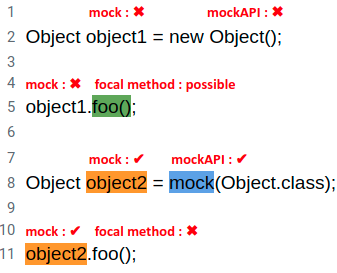
\includegraphics[width=.25\textwidth]{Images/mockFocalMethodIllustration.png}
    
    \caption{Illustration of the process locating mock object and determining non focal method.}
    \label{fig:focalMethodIllustration}
    
\end{figure}

\begin{figure}
    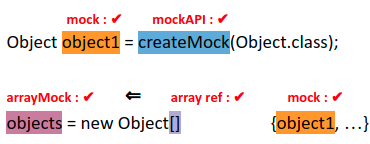
\includegraphics[width=.25\textwidth]{Images/arrayMockIllustration.png}
    
    \caption{Illustration of the process determining array that is an arrayMock.}
    \label{fig:arrayMockIllustration}
    
\end{figure}
